% !TEX program = xelatex

\documentclass[a4paper,14pt,oneside,final]{memoir}
% \usepackage[top=2cm, bottom=2cm, left=3cm, right=1cm]{geometry}
\usepackage{scrextend}

\usepackage{float}
\usepackage{pgfplots}
\usepackage{graphicx}
\usepackage{multirow}
\usepackage{amssymb,amsfonts,amsmath,amsthm}
\usepackage{csquotes}

\usepackage{listings}
\lstset{basicstyle=\footnotesize\ttfamily,breaklines=true}
\lstset{language=Matlab}

\usepackage[
	backend=biber,
	sorting=none,
	language=auto,
	autolang=other
]{biblatex}
\DeclareFieldFormat{labelnumberwidth}{#1}


\usepackage{systeme}
\usepackage{longtable,tabu}
\usepackage{multirow}
\usepackage{array,multirow}
\usepackage{pdflscape}
\usepackage{afterpage}
\usepackage{bm}
\usepackage{framed}

\graphicspath{{figures/}}

\title{Software Design Document}
\author{Artem Chepurnoy}

\begin{document}
\maketitle

\clearpage
\tableofcontents

\chapter{Introduction}
\section{Scope}
This document describes the detailed structure of the components of the Text Tagger and the precise implementations details.

\section{Aim}
The design description defined in this document serves multiple purposes:
\begin{itemize}
    \item To describe the functional structure, data and algorithms to be implemented.
    \item To identify required system resources.
    \item To be used to assess the impact of requirement changes.
    \item To assist in producing test cases.
    \item To aid in maintanance activities.
\end{itemize}

\section{Intended Audience}
Most of this Software Design Description is written for knowledgeable software professionals and designers.
Thus the Client will not be within the intended audience for this document, which is:
\begin{itemize}
    \item Development team.
    \item Supervisor.
\end{itemize}

\section{People}
\subsection{Team}
The team for the project consists of:
\begin{itemize}
    \item Artem Chepurnoy, \texttt{artemchep@gmail.com}.
\end{itemize}

\subsection{Supervisor}
The supervisor for this project is Olga Cherednichenko, contactable at the following email addresses: \texttt{olha.cherednichenko@gmail.com}

\chapter{Module Design}
\section{Architectural Design}
Figure~\ref{fig:class} shown the class diagram for the system.

\begin{figure}[h]
    \centering
    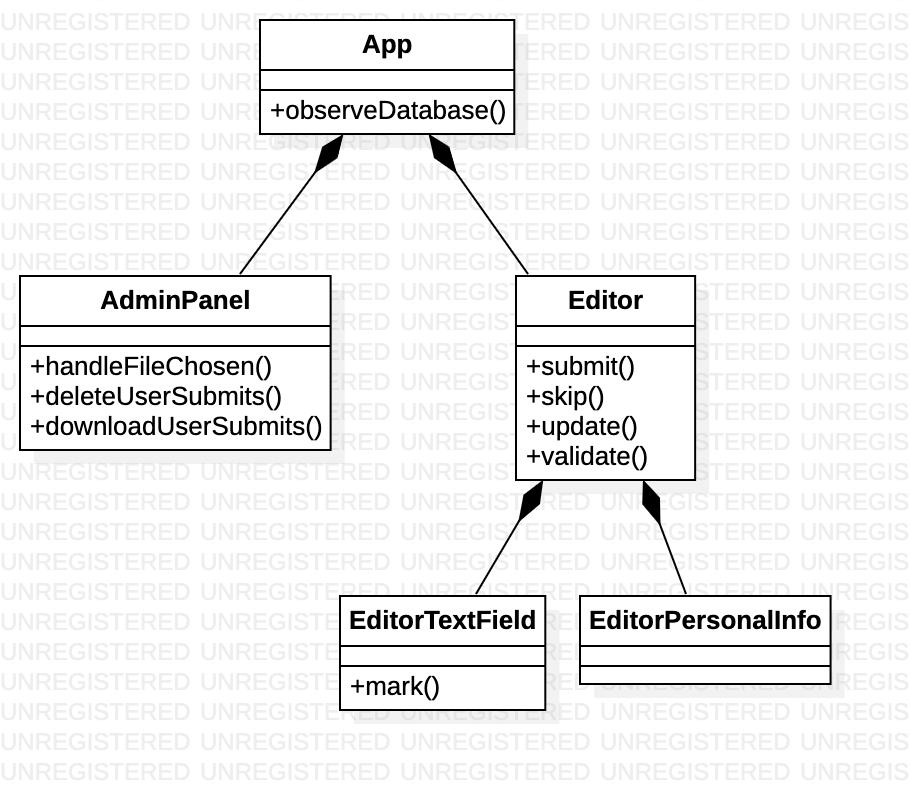
\includegraphics[width=0.7\textwidth]{fig_class}
    \caption{Class diagram of the system}
    \label{fig:class}
\end{figure}

The UI is written using the ReactJS framework in a declarative style. For the database and backend we use Firebase Realtime Database.

\subsection{App class}
Main component of the application, that loads and provides the data from the database, handles page routing.

\subsection{Editor class}
Represents the \texttt{/} (root) route and provides the functionality of entering the user information, marking the text and submitting it to the database. The text to be shown is picked randomly from existing texts.

The component has two child components:
\begin{itemize}
    \item \texttt{EditorTextField}.
    \item \texttt{EditorPersonalInfo}.
\end{itemize}

The description of operations:
\begin{itemize}
    \item \texttt{\#submit()} --- invoked by a click on the <<submit>> button. Invoking the function formats currently marked text, validates user personal info and if it's valid, uploads the text to the database and invokes \texttt{\#update()} function.
    \item \texttt{\#skip()} --- invoked by a click on the <<skip>> button. Invoking the function replaces currently shown text with a new randomly picked one by invoking the \texttt{\#update()} function.
    \item \texttt{\#update()} --- invoking the function replaces currently shown text with a new randomly picked one.
\end{itemize}

\subsubsection{EditorTextField class}
Represents the text field that shows the text and allows user to mark complex words.

\subsubsection{EditorPersonalInfo class}
Represents the personal info fields.

\subsection{Admin Panel class}
Represents the \texttt{/admin-panel} route and provides the functionality of downloading/deleting the user submits and replacing the database of texts with a new one, loaded from the \texttt{.zip} file.

The description of operations:
\begin{itemize}
    \item \texttt{\#handleFileChosen()} --- invoked by the browser when user picks a \texttt{.zip} file from the device. Invoking the function un-archieves the file, replaces all of the forbidden characters with the character '\texttt{\_}' and sends the data to the database.
    \item \texttt{\#deleteUserSubmits()} --- invoked by a click on the <<delete user submits>> button. Invoking the function drops the \texttt{results} collection.
    \item \texttt{\#downloadUserSubmits()} --- invoked by a click on the <<download user submits>> button. Invoking the function loads the data from the \texttt{results} collection and downloads it on the device in \texttt{JSON} format.
\end{itemize}

\section{Design Rationale}
We've chosen the ReactJS as our UI framework of a choice. The advantages of using the ReactJS are: simplicity of use for simple apps, testability and performance. The disadvantage is a high learning curve.

We've chosen the Firebase Realtime Database as our database. The reason was its integration simplicity and realtime support. The disadvantage can be the price of a service for high load applications.

\chapter{Database Design}
\section{Scheme}
We use the key-value database:
\begin{verbatim}
    resources: {
        text_file_name: String
    },
    results: {
        html: String,
        info: {
            academicDegree: String,
            age: String,
            domainExpertise: String,
            languageProficiencyLevel: String,
        },
    },
\end{verbatim}

\section{Field Description}
\begin{itemize}
    \item \texttt{resources} --- contains a collection of texts. 
    \item \texttt{results} --- contains a collection of submitted reports.  
    \begin{itemize}
        \item \texttt{html} --- formatted by user text, where marked as complex parts of the text are marked with the \texttt{<strong/>} tag, for example: \texttt{<strong length-symbols="3" length-words="1">age</strong>}. 
        \item \texttt{info} --- personal information of a user who submitted the text.  
        \begin{itemize}
            \item \texttt{academicDegree} --- user's academic degree, can be one of the following: Doctoral degree, Master's degree, Bachelor's degree, Associate's degree. 
            \item \texttt{age} --- user's age, required to be a number. 
            \item \texttt{domainExpertise} --- user's domain expertise, can be one of the following: Expert, Non-expert.  
            \item \texttt{languageProficiencyLevel} --- user's language proficiency level (in ILR scale), can be one of the following: Native, Professional Working, Limited Working, Elementary, No.  
        \end{itemize}
    \end{itemize}
\end{itemize}

\chapter{Human Interface Design}
This section will detail all aspects of the UI and its design.

The Graphical User Interface (GUI), for the purpose of this description, has been broken up into two main sections. 
These are:
\begin{itemize}
    \item The main screen.
    \item The admin panel.
\end{itemize}

\section{Main screen}
The main screen is shown on figure~\ref{fig:ui_main}. It's available under the \texttt{/} (root) route.

\begin{figure}[h]
    \centering
    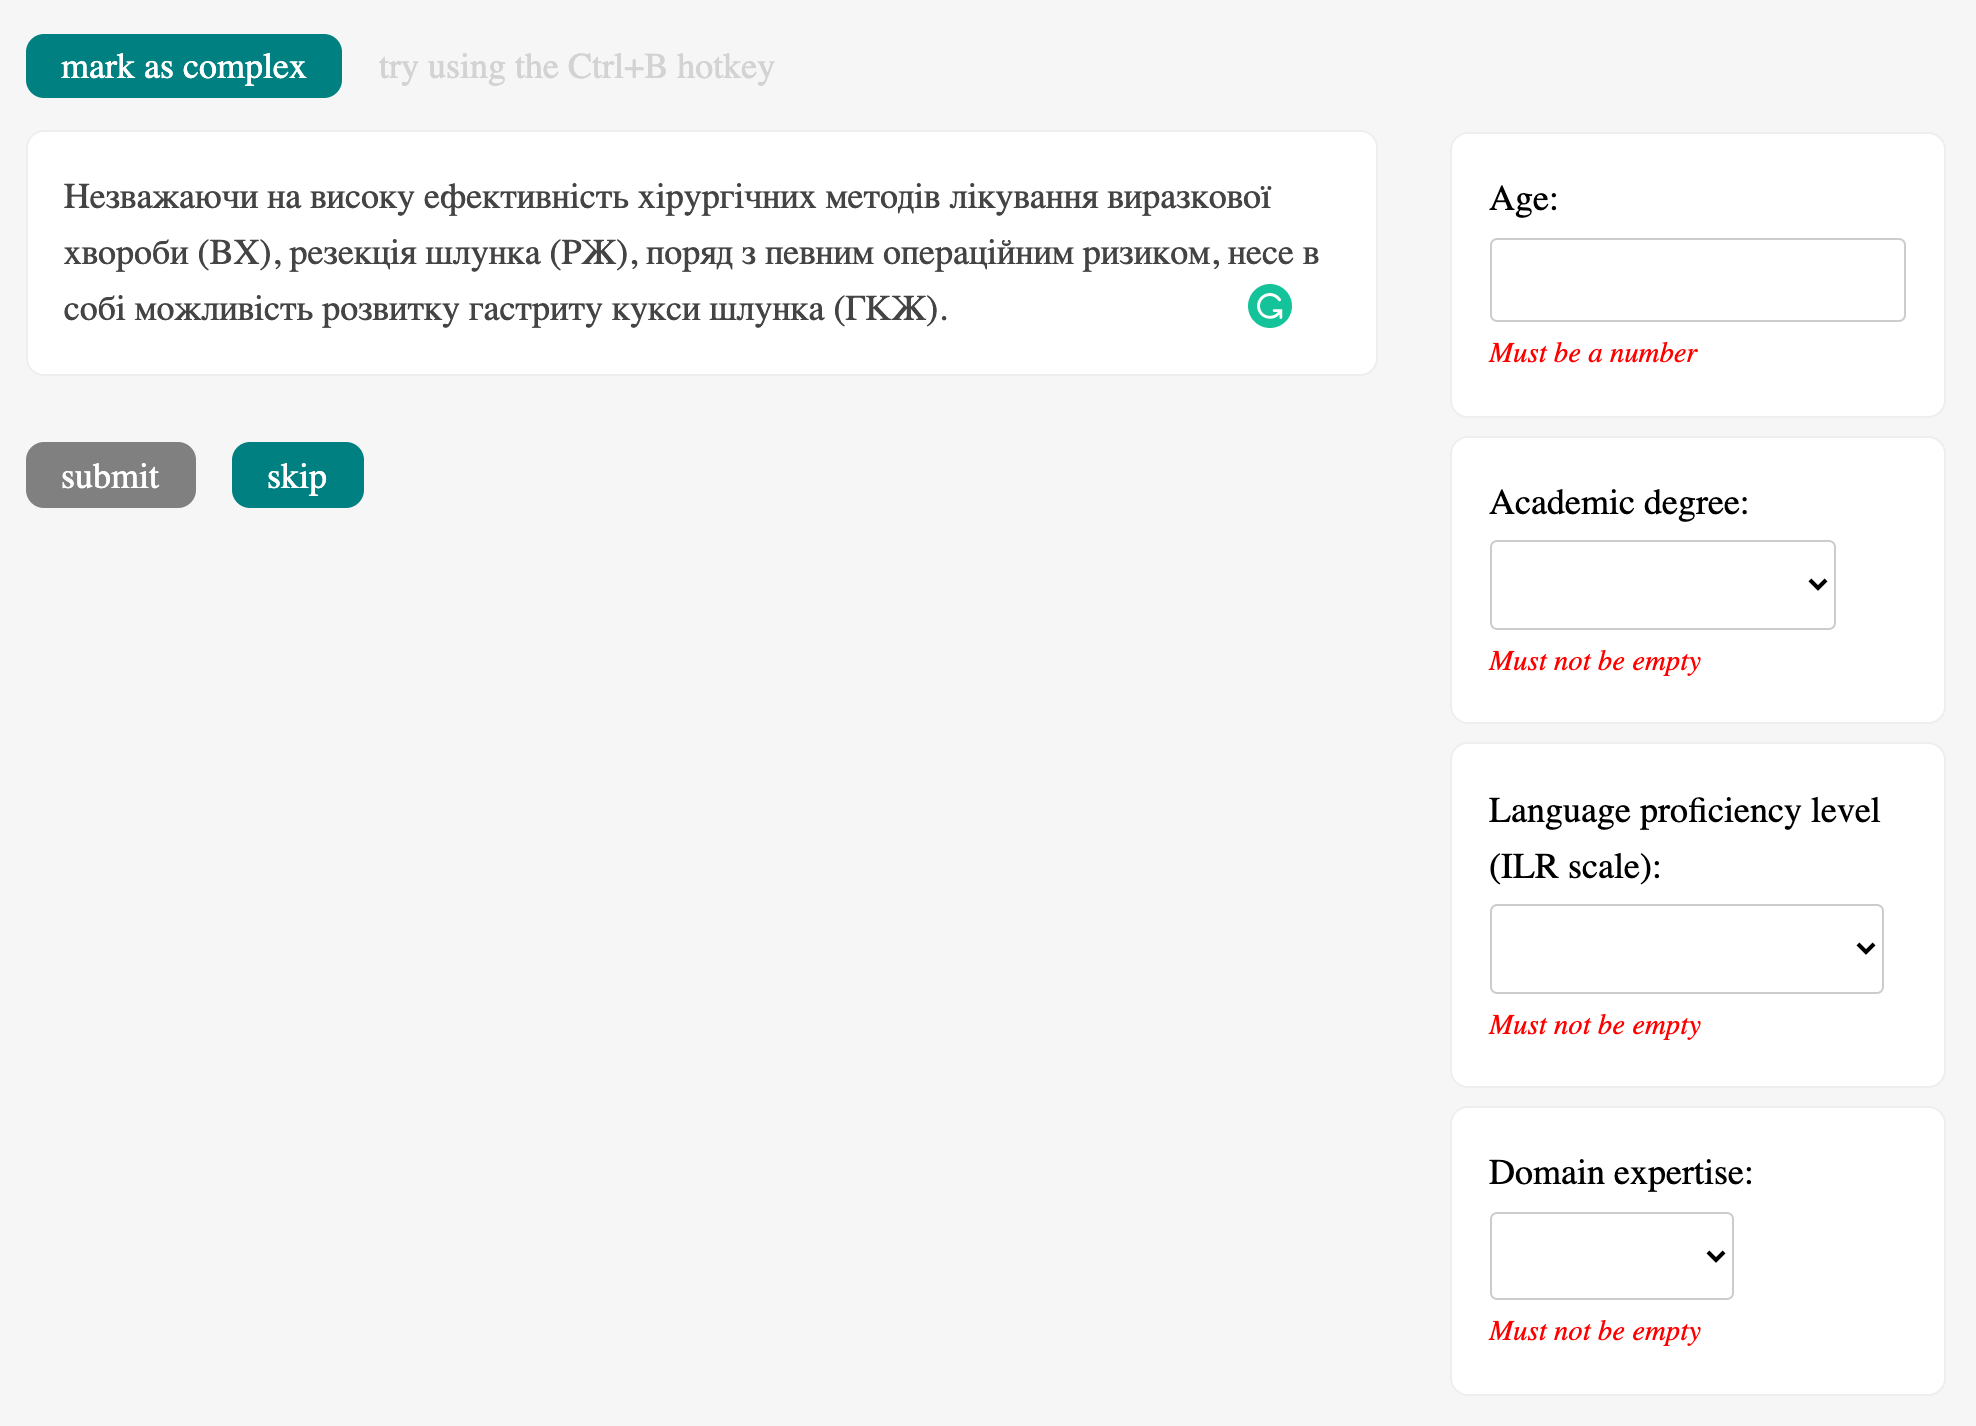
\includegraphics[width=0.7\textwidth]{fig_ui_main}
    \caption{Screenshot of the main screen}
    \label{fig:ui_main}
\end{figure}

The screen can be divided on two components: text editor component and personal info component.

\subsection{Text editor component}
Text editor component consists of four functional elements: 
\begin{itemize}
    \item The <<mark as complex>> button --- marks/un-marks currently selected part of the text as <<complex>>.
    \item The text field --- displays the text and allows user to select parts of the text.
    \item The <<submit>> button --- submits text to the database. Active only if the personal info is valid.
    \item The <<skip>> button --- replaces currently shown text with a randomly picked one.
\end{itemize}

\subsection{Personal info component}
Text editor component consists of four functional elements: 
\begin{itemize}
    \item The <<Age>> field --- lets user to enter his age.
    \item The <<Academic degree>> field --- lets user to enter his academic degree.
    \item The <<Language proficiency level>> field --- lets user to enter his language proficiency level.
    \item The <<Domain expertise>> field --- lets user to enter his domain expertise.
\end{itemize}

All of the elements have a label that shows up if the content of the element is invalid. 

\section{Admin panel}
The admin panel screen is shown on figure~\ref{fig:ui_admin}. It's available under the \texttt{/admin-panel} route.

\begin{figure}[h]
    \centering
    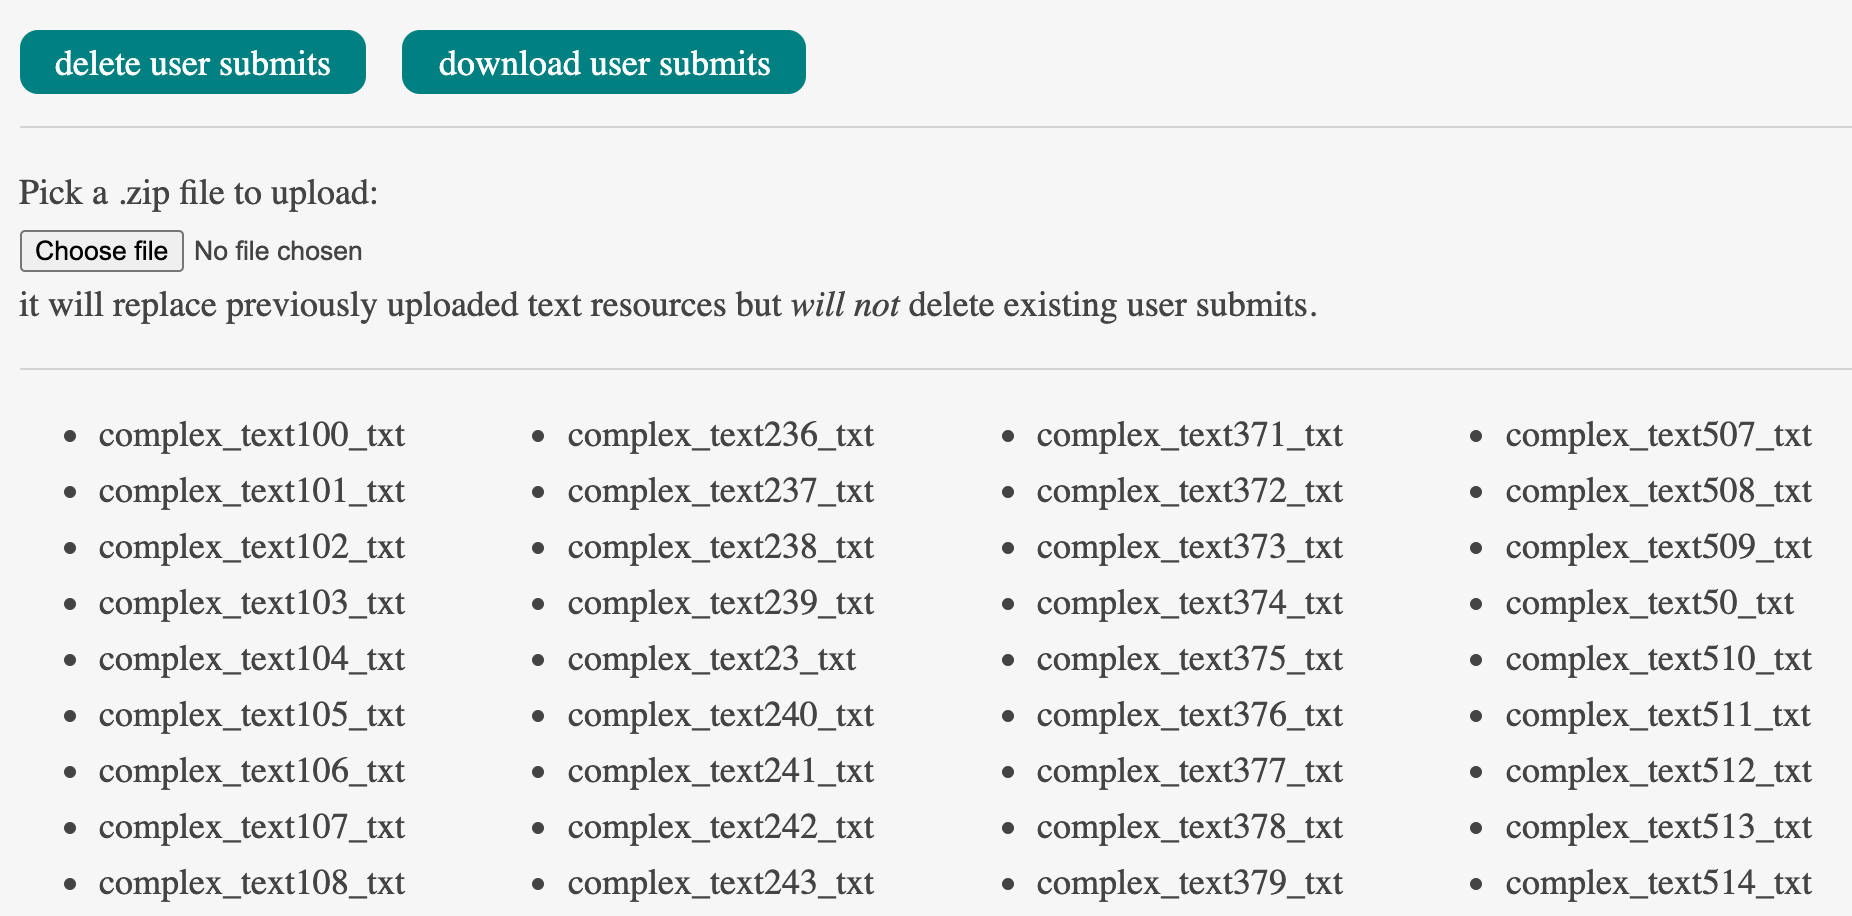
\includegraphics[width=0.7\textwidth]{fig_ui_admin}
    \caption{Screenshot of the admin panel screen}
    \label{fig:ui_admin}
\end{figure}

Admin panel consists of three functional elements: 
\begin{itemize}
    \item The <<delete user submits>> button --- deletes all previously submitted user reports.
    \item The <<download user submits>> button --- downloads all previously submitted user reports.
    \item The <<Choose file>> button --- lets user to upload new database of texts for later marking.
\end{itemize}

On the bottom of the screen all currently active texts are shown. 

\end{document}
